\documentclass[10pt,executivepaper]{article}
\usepackage[utf8]{inputenc}
\usepackage[spanish]{babel}
\usepackage{amsmath}
\usepackage{amsfonts}
\usepackage{amssymb}
\usepackage{graphics}
\usepackage{graphicx}
\usepackage[left=1cm,right=1cm,top=2cm,bottom=2cm]{geometry}
\usepackage{imakeidx}
\makeindex[columns=3, title=Alphabetical Index, intoc]
\usepackage{listings}
\usepackage{xcolor}
\usepackage{multicol}
\usepackage{changepage}
\usepackage{float}
\usepackage{cite}
\usepackage{url}
\usepackage{hyperref}
\usepackage{pdfpages}

\definecolor{codegreen}{rgb}{0,0.6,0}
\definecolor{codegray}{rgb}{0.5,0.5,0.5}
\definecolor{codepurple}{rgb}{0.58,0,0.82}
\definecolor{backcolour}{rgb}{0.95,0.95,0.92}

\lstdefinestyle{mystyle}{
    backgroundcolor=\color{backcolour},
    commentstyle=\color{codegreen},
    keywordstyle=\color{magenta},
    numberstyle=\tiny\color{codegray},
    stringstyle=\color{codepurple},
    basicstyle=\ttfamily\footnotesize,
    breakatwhitespace=false,
    breaklines=true,
    captionpos=b,
    keepspaces=true,
    numbers=left,
    numbersep=5pt,
    showspaces=false,
    showstringspaces=false,
    showtabs=false,
    tabsize=3
}

\lstset{style=mystyle}
\title{Practica 1 Volumen al 50\%}
\newcommand\tab[1][1cm]{\hspace*{#1}}
\begin{document}
  \maketitle
  \section{Descipción de la practica}
  De acuerdo a la descipción proporcionada por el moodle del profesor solicita lo siguiente:
  \begin{center}
    \lstinputlisting[language=C]{solicitud.txt}
  \end{center}
  \clearpage
  \section{Requisitos y saberes previos para realizar la practica}
  Para poder solucionar esta pequeña practica es necesario considerar el tamaño de la cabecera (HEADER) de un archivo WAV, por lo cual a continuación se añadira el header de un archivo WAV
  \begin{center}
    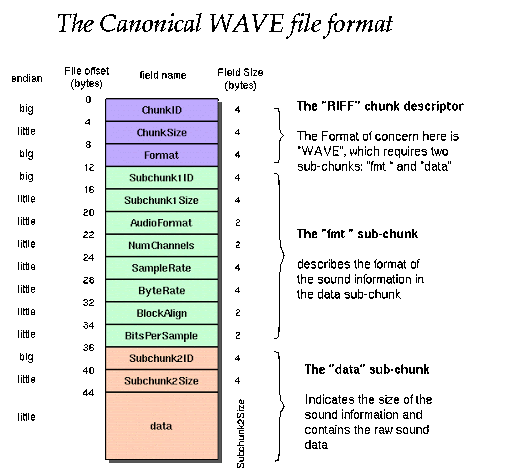
\includegraphics[scale=0.75]{imgs/wavHeader.png}
  \end{center}
  Con esto podremos reconocer que el orden de los primeros $44$ $bytes$ de información por lo que podremos construir la siguente estructura de C
  \begin{center}
    \lstinputlisting[language=C]{sources/headerWAV.h}
  \end{center}
  Una vez teniendo esta idea podremos implementar el siguiente Header llamado $cabeceraWAV.h$, cabe destacar que para la entrega separa e individual del archivo en el examen solo es necesario usar la carpeta "moodle", en cualquier otro caso hacer uso del "Makefile", por lo que es necesario tener cmake instalado para que solo con un simple $\$make$ para que finalmente se pueda generar el archivo del main y solo se realicen pruebas de escritorio.
  \section{Código Fuente}
  \subsection{Makefile}
  \lstinputlisting[language=C]{../Makefile}
  \subsection{Headers}
  \begin{center}
    \lstinputlisting[language=C]{../H/color.h}
    \lstinputlisting[language=C]{../H/cabeceraWAV.h}
  \end{center}
  \subsection{Sources}
  \begin{center}
    \lstinputlisting[language=C]{../C/cabeceraWAV.c}
    \lstinputlisting[language=C]{../C/main.c}
  \end{center}
  \subsection{Código aceptado por Moodle}
  \begin{center}
    \lstinputlisting[language=C]{../moodle/versionExMoodle.c}
  \end{center}



\end{document}
